\section{Evaluation on Aggregate Human Occupancy Behaviour Dataset}
\label{sec:evareal}

We also investigated the performance and practicality of the POPP model and its extensions using switching filters on a large, real world data set. Performance comparison against the FOPP model is now included in this evaluation.

This dataset was gathered from an office building in which a mobile robot counts the numbers of people passing by, as it patrols (see Figure~\ref{fig:map_popp_independent_test} for the map). The data set contains a time series of counts from three different automated person detectors \cite{dondrup2015real}. These use laser, depth camera and RGB information. We refer to them respectively as the leg detector (LD), upper body detector (UBD), and change detector (CD). Each returns a sensed count of the number of people it detected in each 10 minute interval during the day. These detectors are unreliable, as can be seen from Figure~\ref{fig:single_sensor_rate_transformation}, which shows examples of correct and incorrect detections.

\begin{figure}[t]
	\centering
	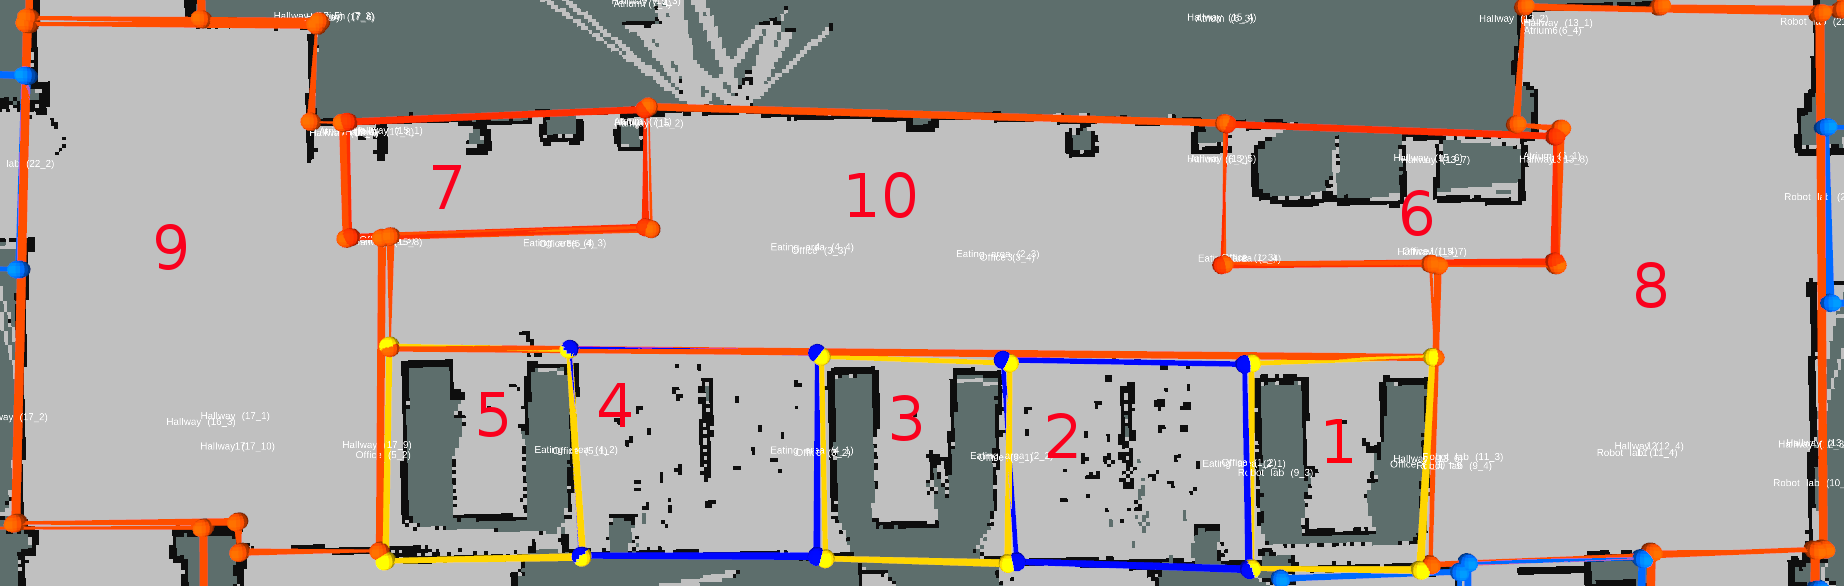
\includegraphics[width=0.95\columnwidth]{./figures/map_popp.png}
	\caption{The office building in which the robot gathered data. Areas are bounded by imaginary lines.}
	\label{fig:map_popp_independent_test}
\end{figure}

\begin{figure}[t]
	\centering
	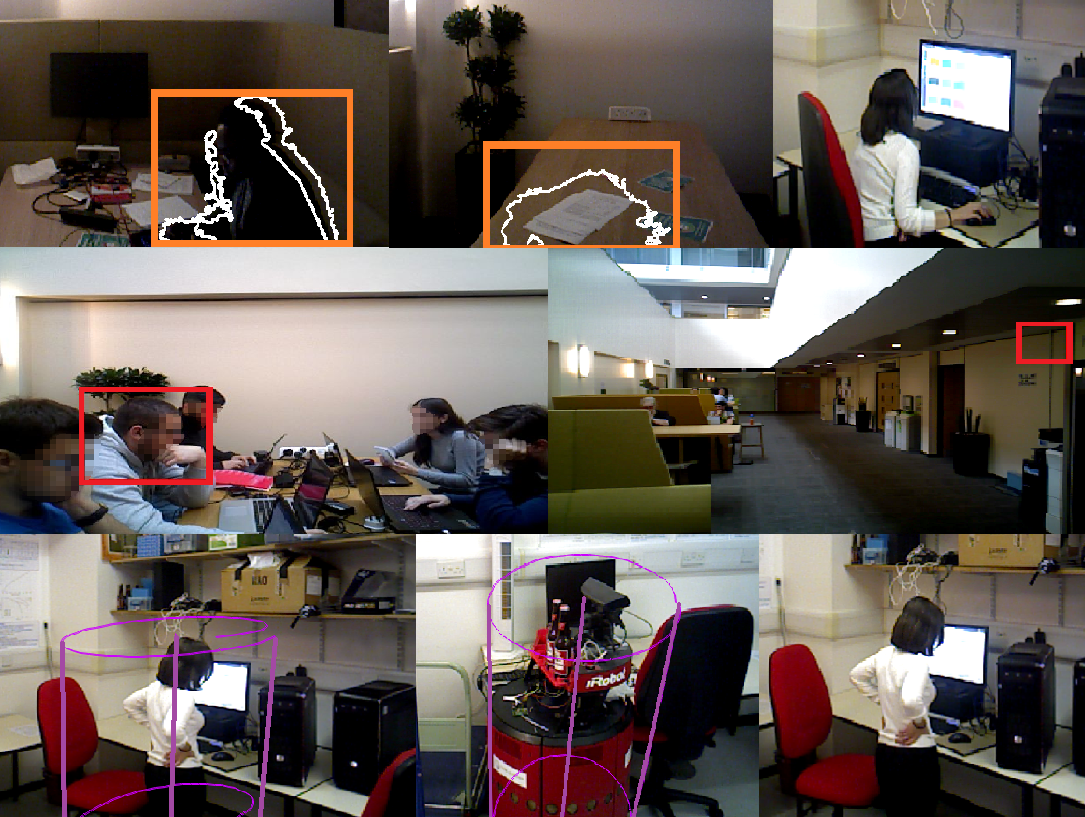
\includegraphics[width=0.95\columnwidth]{./figures/sensor_images.png}
	\caption{Correct and incorrect detections (and non-detections) from different regions in the environment for each sensor. Top row: change detector. Middle row: upper body detector. Bottom row: leg detector. Detections are marked with 2D or 3D bounding boxes.}
	\label{fig:single_sensor_rate_transformation}
\end{figure}

By comparing the ground truth with the detections made by sensors, we calculated a sensor unreliability model for each region. An average of a sensor model across different regions can be seen in Table \ref{table:sensor_model_popp_beta}. Although the robot operated 24/7, the sensor models were built using the data collected from 10am-8pm, there being negligible detections outside these times. From a 69-day deployment of the mobile robot, we obtained 48 days of usable observations. We specified a time interval for each Poisson distribution of 10 minutes, and recorded both the true counts and the detections made by each sensor in each interval. We assumed that the underlying process on each region to be a periodic Poisson process in which there is a one-day periodicity cycle, i.e. $\lambda(t) = \lambda(t + \Delta)$ with $\Delta = 24 * 60$(minutes), on the process. This means that the expected number of people turning up on each day in particular time of the day is the same across the 48 days of observations. We then estimated the true parameter $\lambda(t)$ of the Poisson distribution at $t$ interval by running a FOPP model on the true counts within the $t$ interval.

The different POPP models rely on sensor models that must be calculated from a confusion matrix relating true counts and the different sensor counts. To separate the training and testing data we performed four fold cross-validation with the unit being whole days, i.e., we used 12-days of data as a training set for a sensor model and then used the remaining 36-days of data as a test set on which to test the inferences made by each model from the sensor counts.

\begin{table}[t]
	\centering
	\caption{Averaged sensor model across all areas trained from 48 days of data.}
	\label{table:sensor_model_popp_beta}
	\begin{tabular}{lccc}
		\noalign{\hrule height 1.1pt}\noalign{\smallskip}
		Sensor & True Positive & True Negative \\
		\noalign{\smallskip}\hline\noalign{\smallskip}
		Leg Detector & 0.387 & 0.951 \\
		Upper Body Detector & 0.356 & 0.882 \\
		Change Detector & 0.731 & 0.900 \\ 
		\noalign{\hrule height 1.1pt}\noalign{\smallskip}
	\end{tabular}
\end{table}

For the 36 days of test data the different models each made predictions of the $\lambda(t)$ parameter of the Poisson. Given this, we recorded (1) a distance metric method using the RMSE of the MAP hypothesis of each model posterior distribution over $\lambda(t)$ to the true $\lambda'(t)$ and (2) a free-distance metric method using the Jensen-Shannon distance between the posterior distribution $P(\lambda(t) ; \overrightarrow{s_i})$ and the distribution of the true $\lambda'(t)$ generated from the FOPP model on true counts. Using these metrics, we compared the performance of all POPP models, using the switching filter, to the standard Bayes' filter arising from the FOPP model. The uncorrected estimate $\lambda(t)$ according to the FOPP model was estimated only from the change detector count data since the change detector is the most reliable detector among three detectors available in the robot as shown in Table \ref{table:sensor_model_popp_beta}.

Figure \ref{fig:fopp_popp_popb_npop_popd_rmse_evo} and \ref{fig:fopp_popp_popb_npop_popd_kl_evo} show the accuracy comparison between all POPP models and the standard FOPP model over time in a distance metric method, i.e., RMSE, and a free-distance metric method, i.e., the Jensen-Shannon distance. It can be seen that all models became more and more accurate towards the true $\lambda'(t)$ as days pass by. All POPP models show more accuracy over the standard FOPP model. The $\lambda(t)$ estimate produced by the POPP-Dirichlet model is more accurate than the ones produced by the standard POPP model and the POPP-Beta model. However, the estimate is not always more accurate compared to the one produced by the C-POPP model. 

As the POPP-Dirichlet model is more conservative in estimating the parameter $\lambda(t)$ than the C-POPP model, the estimate moves rather slowly towards the true $\lambda'(t)$. This is showcased by figure \ref{fig:fopp_popp_popb_npop_popd_kl_evo}.
By the third day, the POPP-Dirichlet model outperformed the POPP and the POPP-Beta, and the C-POPP models in terms of accuracy. However, the accuracy gap between the C-POPP model and the POPP-Dirichlet model became smaller and by the 36th day, the C-POPP model outperformed the POPP-Dirichlet by a small margin.

\begin{figure}[t!]
	\centering
	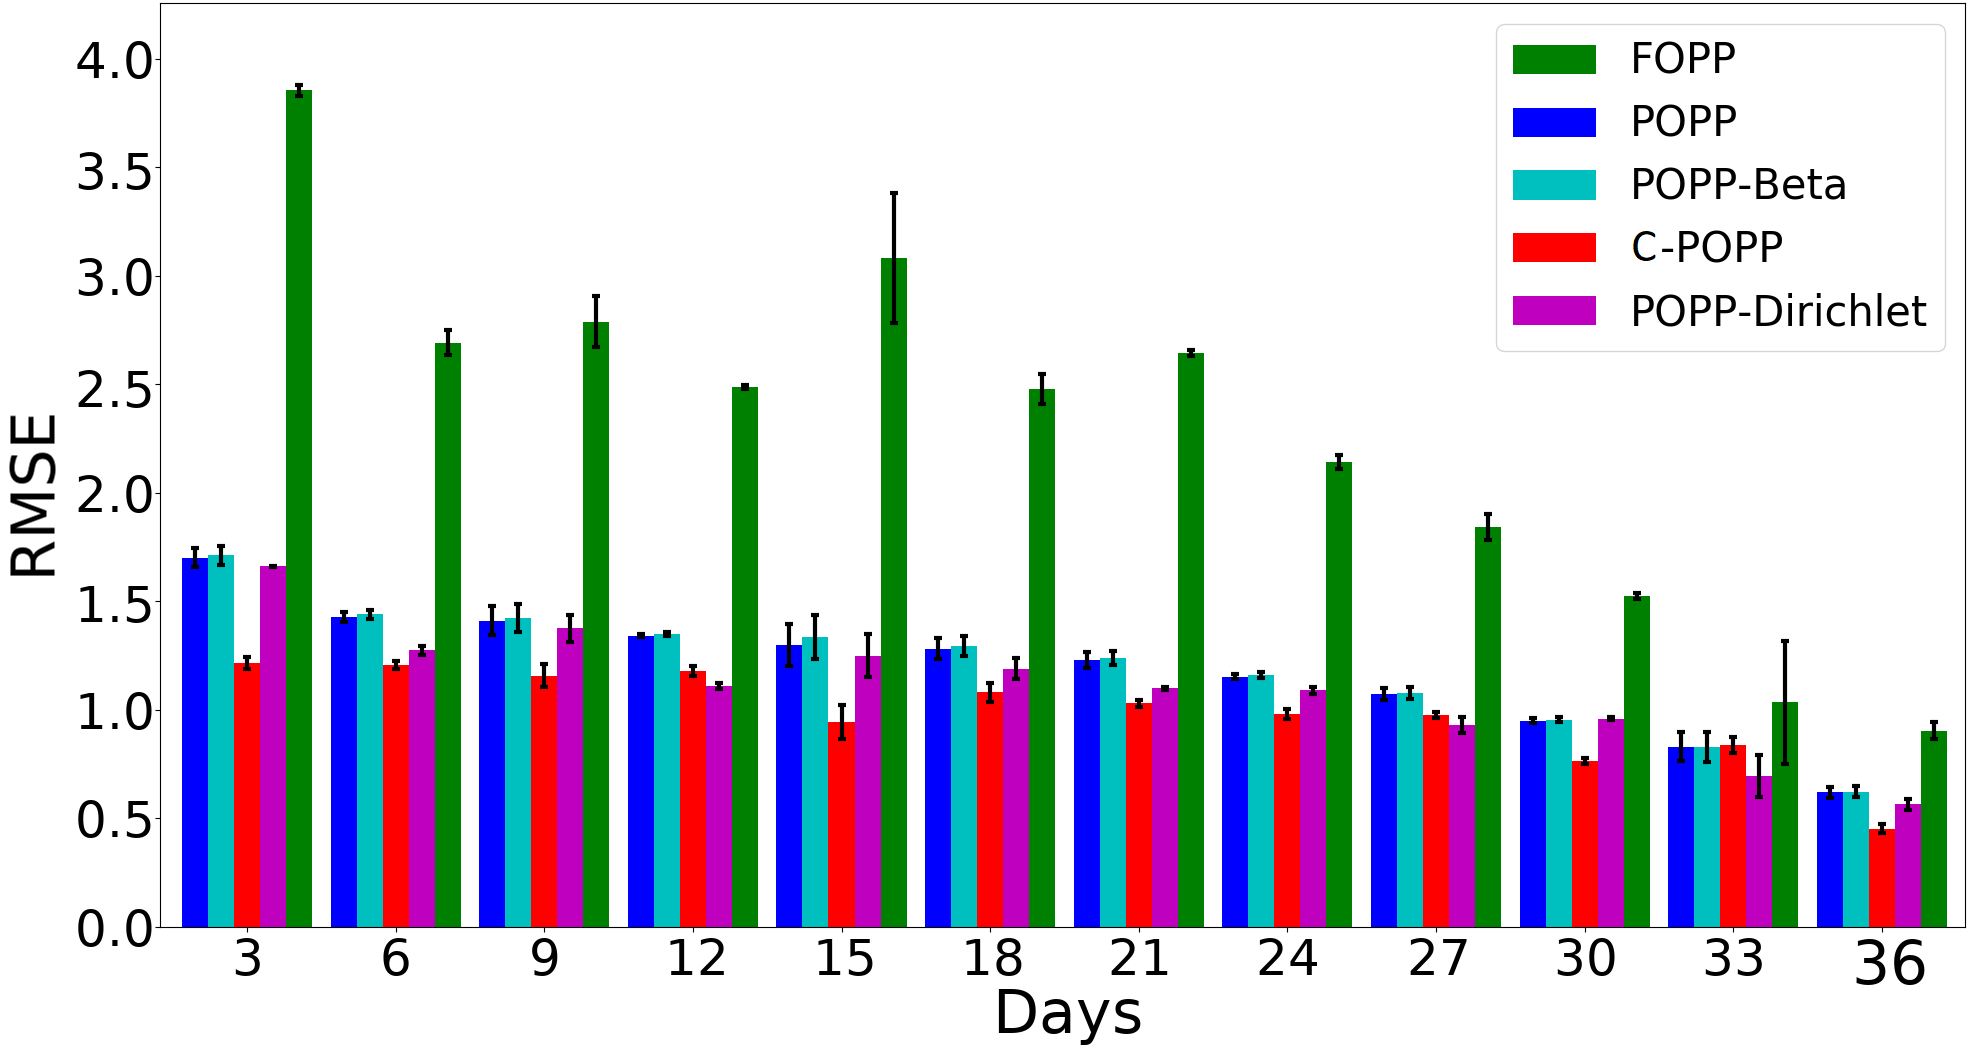
\includegraphics[width=0.95\columnwidth]{./figures/fopp_popp_popb_npop_popd_rmse_evo.png}
	\caption{The RMSE evolution of periodic Poisson processes with POPP, POPP-Beta, C-POPP, POPP-Dirichlet and FOPP filters from day 3 to day 36, averaged across all regions. Standard error is shown.}
	\label{fig:fopp_popp_popb_npop_popd_rmse_evo}
\end{figure}

\begin{figure}[t!]
	\centering
	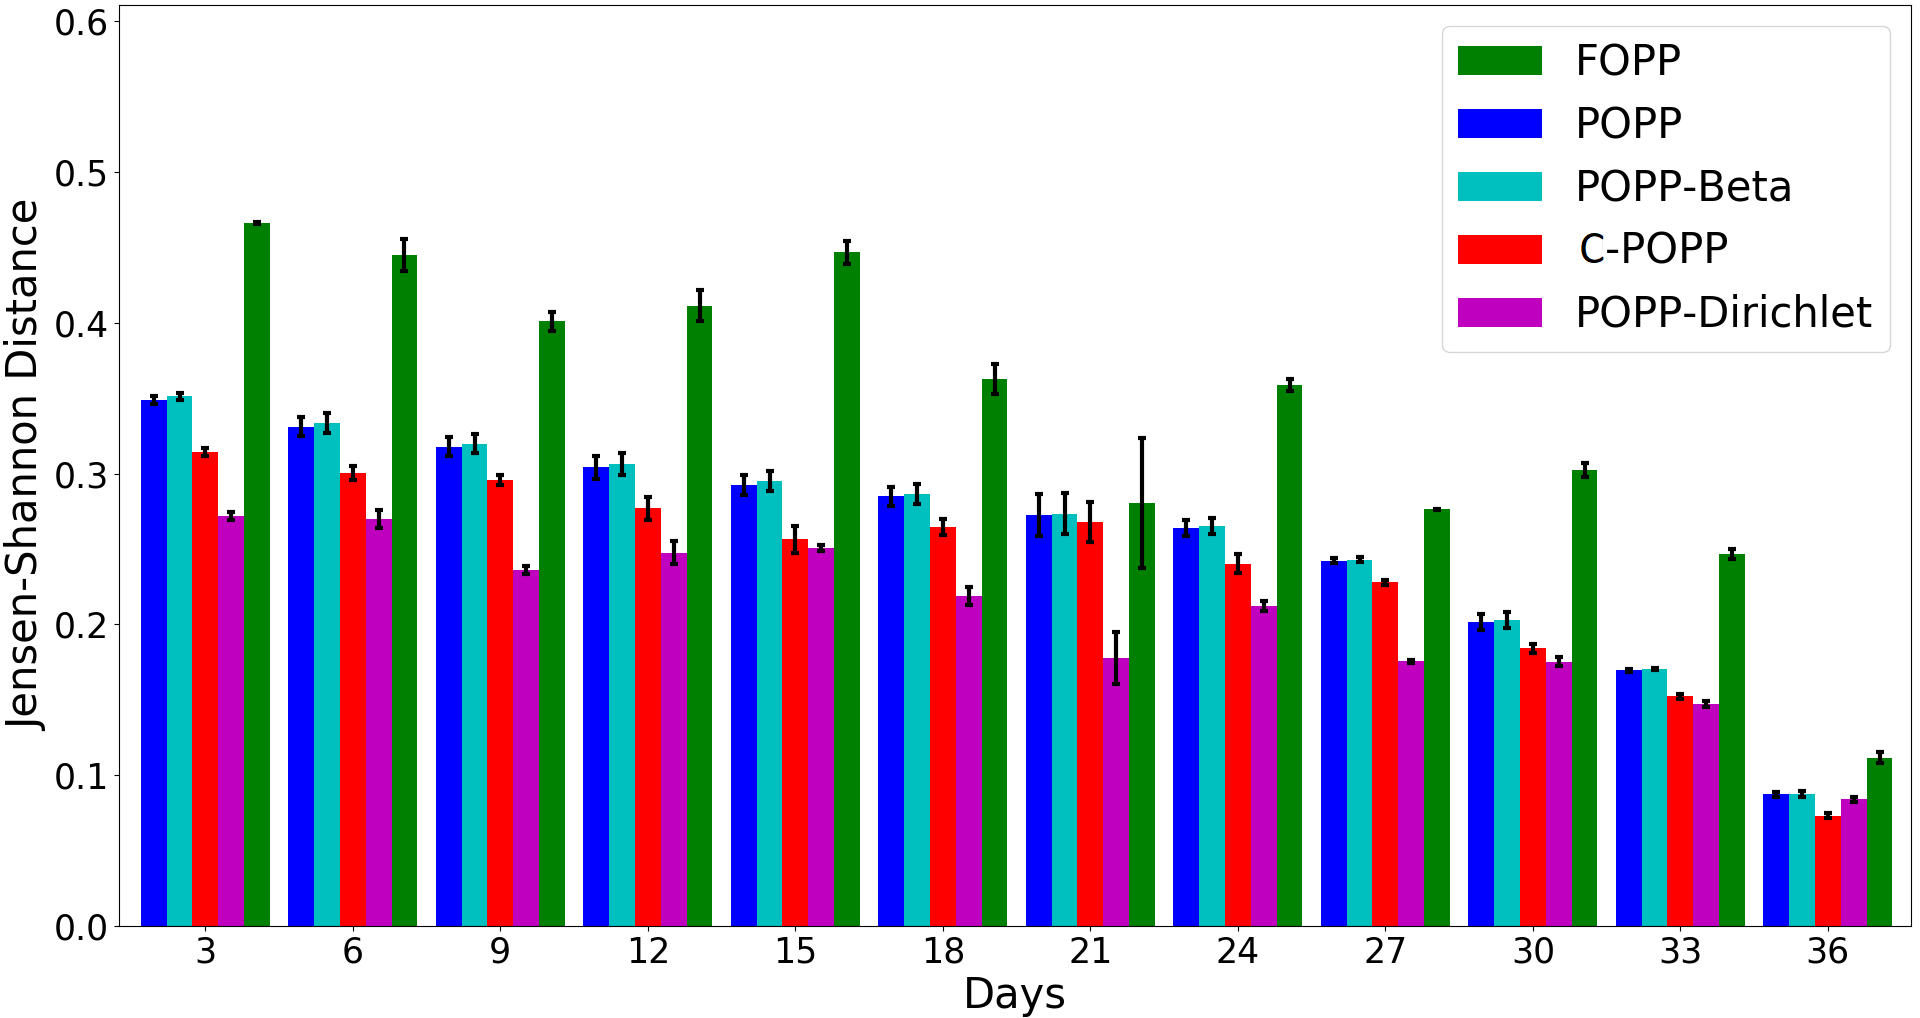
\includegraphics[width=0.95\columnwidth]{./figures/fopp_popp_popb_npop_popd_kl_evo.png}
	\caption{The Jensen-Shannon distance evolution of the FOPP, the POPP, the POPP-Beta, the C-POPP, and the POPP-Dirichlet filters in periodic Poisson processes from day 3 to day 36 in a 3-day interval, averaged across all regions. Standard error is shown.}
	\label{fig:fopp_popp_popb_npop_popd_kl_evo}
\end{figure}

%Similar to the C-POPP model, the POPP-Dirichlet model is able to cope and overcome the problems with limited sample data both for building the joint sensor model and estimating the $\lambda(t_i, t_j)$. In many regions, the POPP-Dirichlet managed to show better estimates as well as more similar distributions than the POPP, the POPP-Beta, and the FOPP models. However, the POPP-Dirichlet filter falls behind both in accuracy (RMSE) and distribution similarity compared to the C-POPP model. This is attributed to the POPP-Dirichlet conservative way in estimating the parameter $\lambda(t_i, t_j)$ compared to the C-POPP model.